\documentclass[11pt,a4paper]{article}
\usepackage[top=3cm, bottom=3cm, left=2.5cm, right=2.2cm]{geometry} %geometry of page
\usepackage[hidelinks]{hyperref} %reference links
\usepackage{fancyhdr} %header and footer control
\usepackage{minted} %source code syntax highlighting
\usepackage{qrcode} %qrcode links
\usepackage{graphicx} %images

\linespread{1.3}
\emergencystretch 3em

% Set Header and Footer
\fancyhead{}
\fancyhead[L]{\textbf{Lab 3: Servo}}
\fancyhead[R]{d.s.brennan@sheffield.ac.uk}
\fancyfoot{}
\fancyfoot[L]{\thepage}
\fancyfoot[R]{MAC 233 Arduino Labs, School of MAC, University of Sheffield}

% Create Document
\begin{document}
\pagestyle{fancy}

\section*{Prerequisites}
This worksheet builds upon the theory of how to use an external pin that was covered in the Lab 2 worksheet. Whilst you won't need any code from Lab 2, you will need to have covered how to use an electronic breadboard and how to wire up an external output to an Arduino pin. Out of your Arduino pack, you will need: 1 Arduino, 1 Servo, and 3 jumper cables.

\section*{Objectives}
The objective of today's lab is to learn how to control a servo using the inbuilt Arduino Servo Library: \url{https://docs.arduino.cc/libraries/servo/}.\\

\noindent
This worksheet will take you through the steps of how to connect an external servo to your Arduino and create a sketch that rotates the servo in increments of 30 degrees. Once the sketch reaches 180 degree (the maximum number of degrees on a servo), the sketch will reset the degrees to zero and start incrementing in steps of 30 degrees again.

\section*{Understanding how a servo works}
Within the remit of this lab, a servo (or servomotor) is a physical device used to control rotary motion. On an Arduino, servos (and some other analogue devices) need to be controlled using Pulse Width Modulation (PWM). You have covered the theory of PWM in last week's electronic lecture; therefore, this lab will not go into detail about PWM (for more details see: \url{https://docs.arduino.cc/learn/microcontrollers/analog-output/}). It is important to understand that depending on the Arduino you are using, not every pin can be used for PWM output. On the Arduino Nano Every, the digital pins that can handle a PWM output are pins: 3, 5, 6, 9, 10 (these details can be viewed from the datasheet linked in lecture 1.)\\

\noindent
On an Arduino there is an inbuilt Servo library that encapsulates the PWM complexities and helps us control a servo (or an Electronic Speed Controller connected to a DC motor). For this library, you simply write an output value to your servo between 0 and 180 --- which maps directly to the number of degrees of rotation available on most servos: 0\textrightarrow 180.\\

\noindent
A servo has three wires coming out of it: a \textit{power} cable, a \textit{ground} cable, and a \textit{signal} cable. The power cable is usually red, the ground cable is usually black or brown, and the signal cable is usually white or orange.

\section{Creating the circuit}
The circuit needed for this worksheet is: Arduino Pin D9\textrightarrow Servo sensor cable, Arduino GND\textrightarrow Servo ground cable, and Arduino +5V\textrightarrow Servo power cable.\\

\section{Setup the servo library}
The first thing we need to do is create a blank sketch, this is done by opening Arduino IDE, going to `File'\textrightarrow `Examples'\textrightarrow `01.Basics'\textrightarrow `BareMinimum'. Once this has opened, we can now setup the Servo library.\\

\noindent
In the global scope (the top of the file), enter in the code below. This code firstly links our sketch to the servo library, then defines a new named pin called `$SERVO\_PIN$' on pin D9, and then creates an instance of the servo library for us to interact with called `servo'.\\
\vspace{-1.75em}
\inputminted{arduino}{./src/1-servo-library.txt}
\vspace{.75em}

\noindent
The next step is for us to declare the array (vector) of integer values we want the sketch to output. For simplicity, we will say for the time being that should be every 30 degrees from 0 to 180. The code below needs to be put into the global scope below the previous code. This code operates on the same logic as Lab 1 and Lab 2; however, instead of having an array of dots and dashes, we now have an array of degrees to rotate the servo to.\\
\vspace{-1.75em}
\inputminted{arduino}{./src/2-degree-list.txt}
\vspace{-.5em}

\section{Setup function}
In the setup function of the sketch, we need to do three things: 1 - setup the standard debugging tools, 2 - set the position in the output, 3 - set the output pin and attach it to the servo library. The code in the following sections, needs to go into the `setup' function.\\

\subsection{Setup debugging}
The first thing to do in any sketch, is to setup the debugging by connecting the Serial. This allows us to monitor what the Arduino is doing via displaying specific messages at certain points throughout the sketch. This code attaches the serial, pauses the system for 3 seconds, and displays a message `System Ready'.\\
\vspace{-1.75em}
\inputminted{arduino}{./src/3-setup-debug.txt}
\vspace{-.5em}

\subsection{Setup output}
In the global scope, we have already declared the desired output; however, it is always good practice to set any variables that could be changed at different points during the sketch. In our case, this is simply setting the current position in the degree output.\\

\vspace{-1.75em}
\inputminted{arduino}{./src/4-setup-output.txt}
\vspace{-.5em}

\subsection{Setup servo}
In the global scope, we have setup the servo library, but we now need to configure the servo library to talk to the correct pins. In our case this is pin D9 that we previously named `$SERVO\_PIN$'. The first thing we need to do is set pin D9 to be an output pin. We can then attach pin D9 to the servo library. Finally, we can set the servo to 0 degrees.\\

\vspace{-1.75em}
\inputminted{arduino}{./src/5-setup-servo.txt}
\vspace{-.5em}

\section{Loop function}
Now that we have the setup function sorted, we can concentrate on the loop function. Within the loop function, there are three major steps: 1 - write the correct value to the servo, 2 - determine the next position in the `output' array, 3 - wait two seconds before the next iteration. The code in the following sections, needs to go into the `loop' function.\\

\subsection{Output to servo}
At the top of the `loop' function, needs to be the logic to write the correct value within the output to the servo. Thankfully, this is one line of code. We need to access the current position within the output array and then tell the servo to use that value. We also add in an additional line here, to output to the serial connection the selected value so that we can monitor the progress of the sketch.\\ 

\vspace{-1.75em}
\inputminted{arduino}{./src/6-loop-write.txt}
\vspace{-.5em}

\subsection{Determine next position}
The next logic within the `loop' function, is the logic to determine the next position within the output array. Thankfully, this is the same logic that is used to determine the next position within the dots and dashes array in Lab 1.\\

\vspace{-1.75em}
\inputminted{arduino}{./src/7-loop-next.txt}
\vspace{-.5em}

\subsection{Wait}
The final logic within the `loop' function, is to wait two seconds until the next iteration. This is done by telling the Arduino to wait 2000 milliseconds.\\

\vspace{-1.75em}
\inputminted{arduino}{./src/8-loop-sleep.txt}
\vspace{-2em}

\section*{Try it out on your Arduino}
You now should be able to compile your sketch (`Sketch'\textrightarrow `Verify/Compile') and then upload to your Arduino (`Sketch'\textrightarrow `Upload'). You should see that your Arduino now rotates your servo 30 degrees every 2 seconds until it gets to 180, at which point it restarts back from 0.\\

\noindent
Once you have a working sketch from the above code, expand the sketch to rotate in 30 degree increments from 0 to 180 and then rotate in 30 degree decrements from 180 back down to 0 without repeating two identical degree values in a row.

\pagebreak
\section*{Help}
If you are having issue compiling the project or don't understand where each section goes, you can see a complete version of the sketch with additional source code comments at \url{https://github.com/dsbrennan/mac-233-arduino-labs/blob/main/lab-3-servo/lab-3-servo.ino}.

\vspace{2em}

\begin{center}
    \qrcode[hyperlink, height=4cm]{https://github.com/dsbrennan/mac-233-arduino-labs/blob/main/lab-3-servo/lab-3-servo.ino}
\end{center}

\vspace{2em}

\noindent
Additionally, if you are wondering how to wire up the circuit required for this lab on the breadboard, the electronic wiring diagram is below.

\begin{center}
    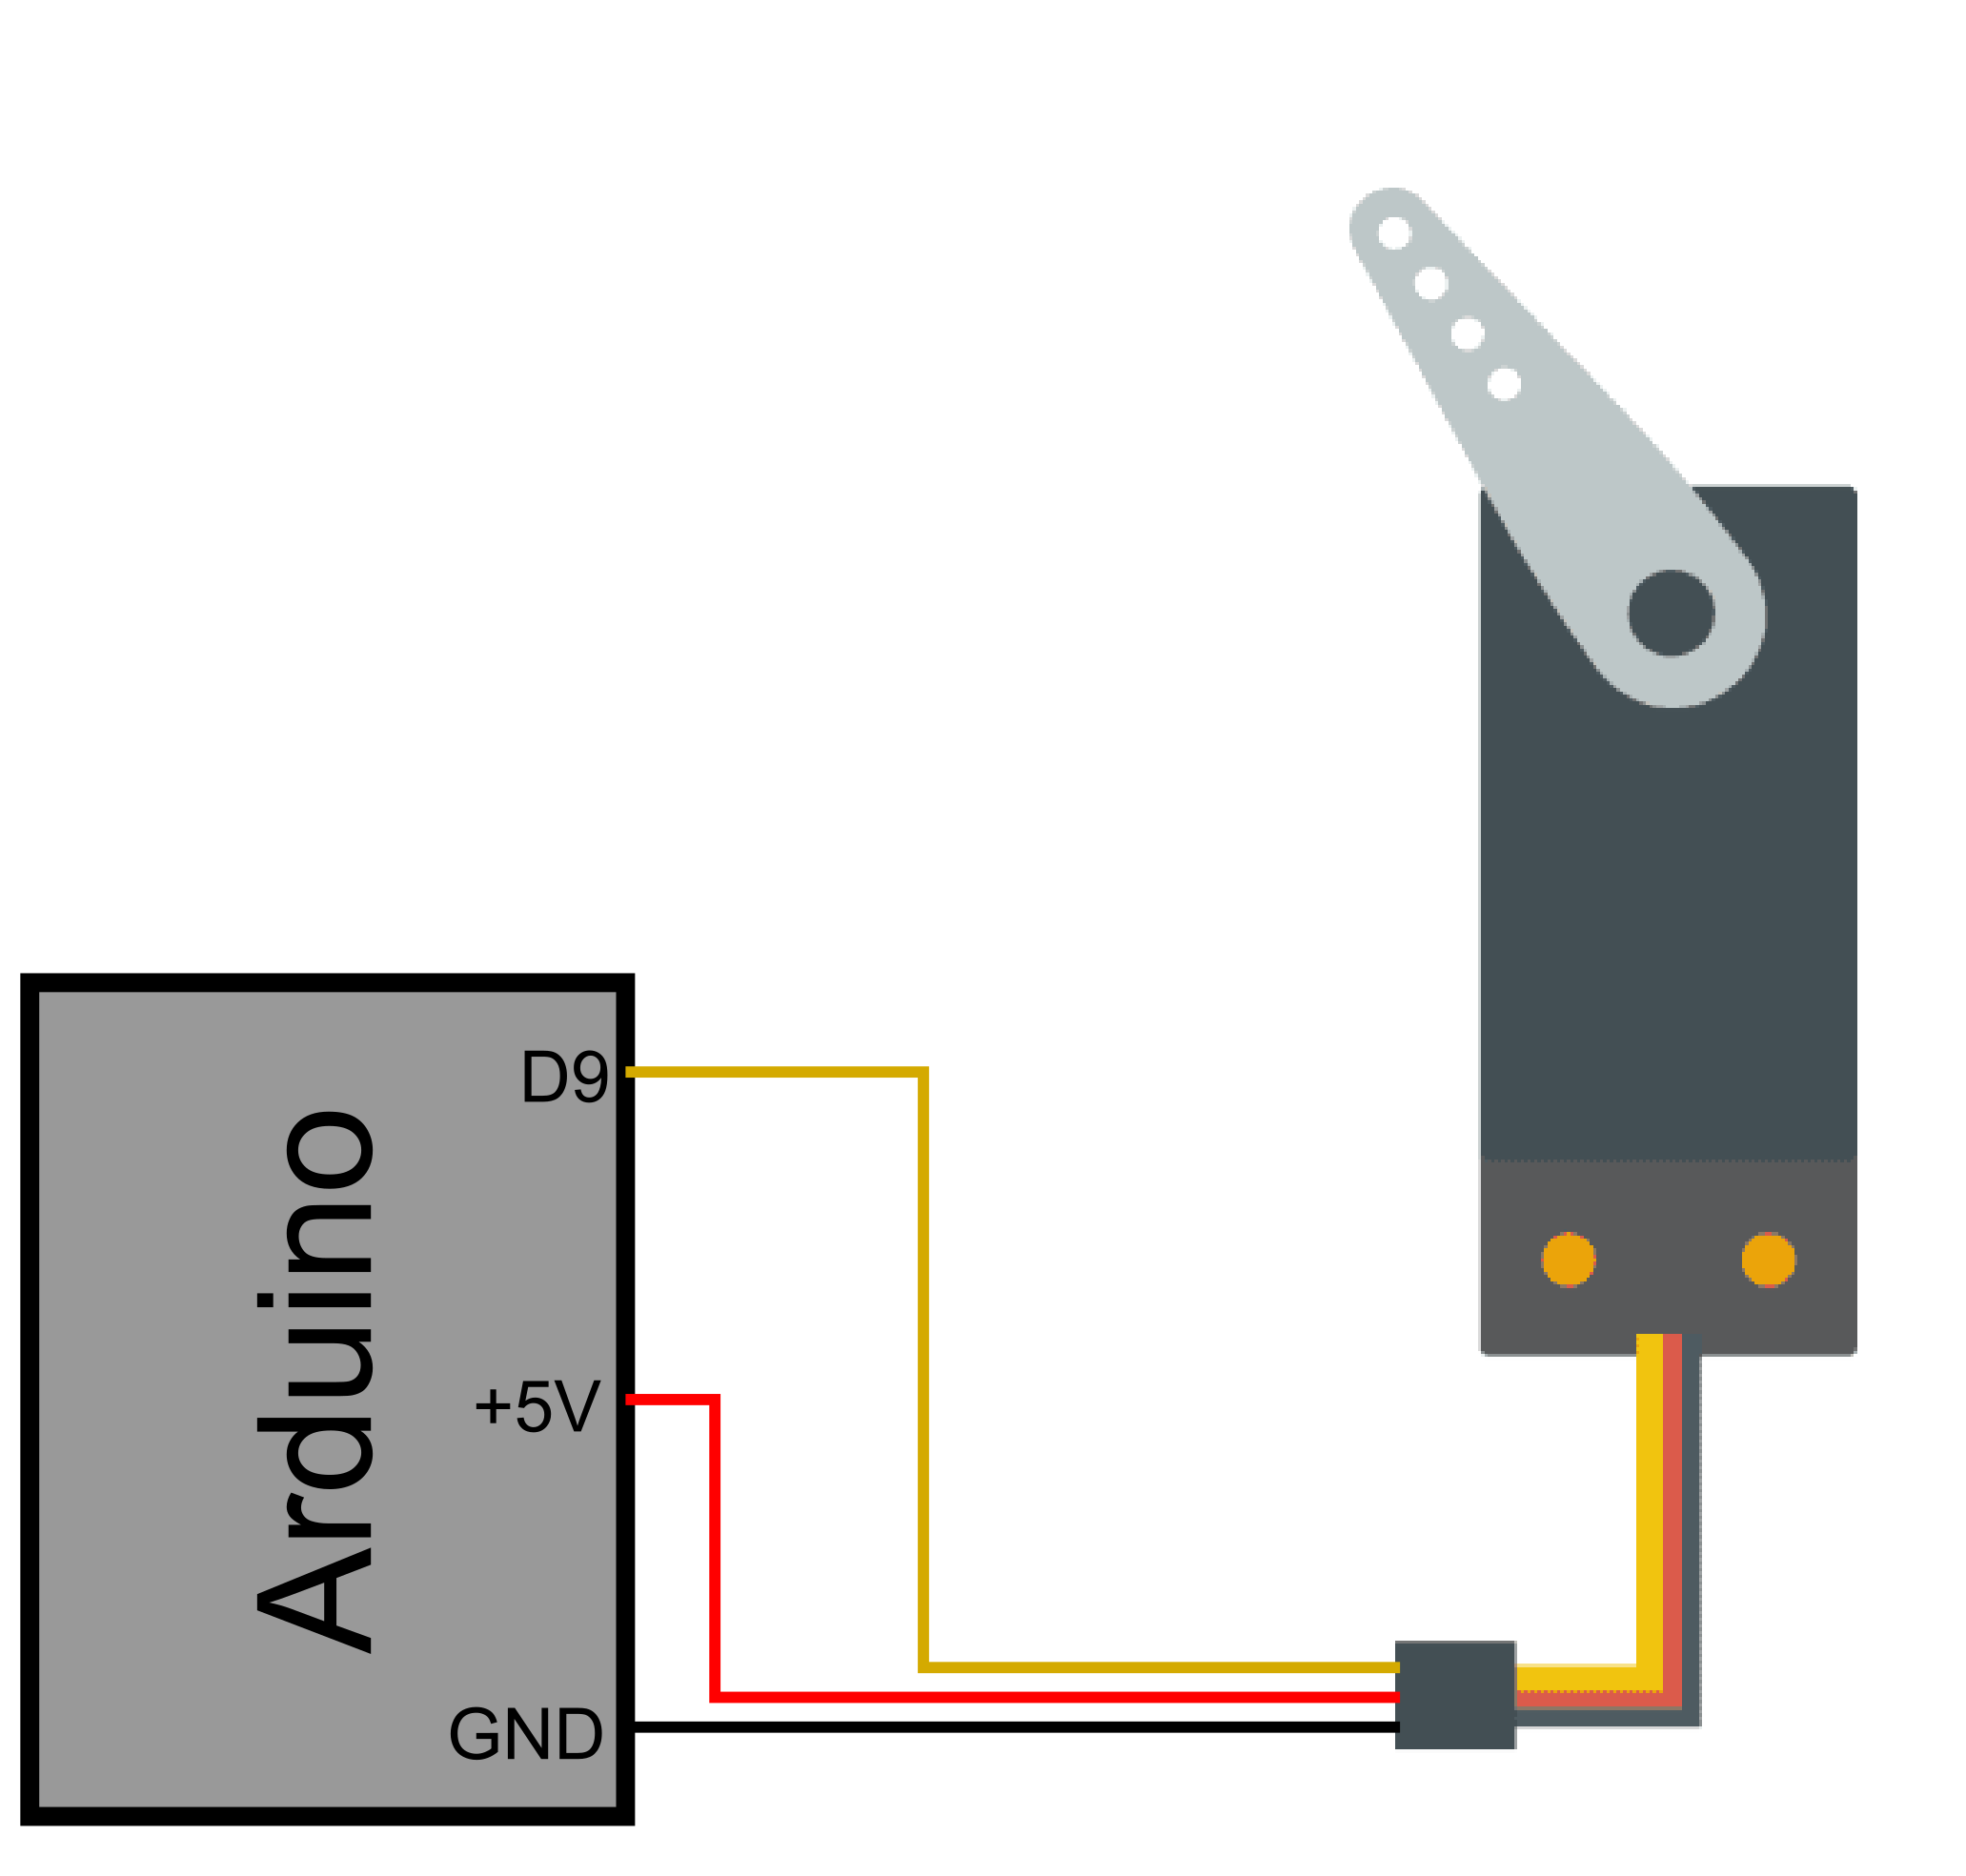
\includegraphics[width=.5\textwidth]{./images/wiring-diagram.png}
\end{center}

\end{document}